% Drawing 80/01-10 -- folder 80, batch 01, archive page 20 (PDF page 21).
% Transcription: en haut de la feuille, quatre dessins d'arrangements de droites, un double trait vertical après le premier : (1) quatre droites en position générale, avec « $4$ » et « $(\mathfrak{S}_4)$ » ; (2) cinq droites en position générale, « $(D_5)$ $5$ pos.\ générale » ; (3) cinq droites dont trois concourantes, « $5$ position particulière » ; (4) six droites, les côtés d'un triangle et trois droites issues des sommets concourantes en un point intérieur, quatre points marqués, « $6$ en position particulière »
% Kind: four small line arrangements (4, 5, 5 and 6 lines). Method 2 (schematic redraw from the facsimile). Status: ok.
% Notes: Ink. (1) four lines in general position. (2) five lines in general position. (3) five lines, three of them through one computed point (the page shows them meeting at one point; this is the special position), one of the three heavy. (4) the three sides of a triangle and the three lines from its vertices through one interior point, all drawn through the four computed points, which are marked. The captions are set as he wrote them; the struck sign between (2) and (3) is not drawn. Redrawn 2026-11-12 (issue 128): to check again.
% Coordinates: 1 unit = 1 mm = 1/100 of the crop width (bbox in page fractions: [0.1, 0.07, 0.96, 0.23]).
% Redrawn by Claude (claude-fable-5-2), issue #128, 2026-11-12; not checked by a human; not compiled (no TeX in the session).
% Rights: reproduces part of the work -- behind RENDER_TRANSCRIPTS, never published by itself.
\documentclass[tikz,border=3pt]{standalone}
\usepackage{amsmath,amssymb}
\usetikzlibrary{patterns,arrows.meta}
\tikzset{pencil/.style={black!45}, struck/.style={black!35}, mpt/.style={circle,draw,inner sep=1.3pt}, pt/.style={circle,fill,inner sep=0.9pt}, opt/.style={circle,draw,fill=white,inner sep=1.1pt}}
\begin{document}
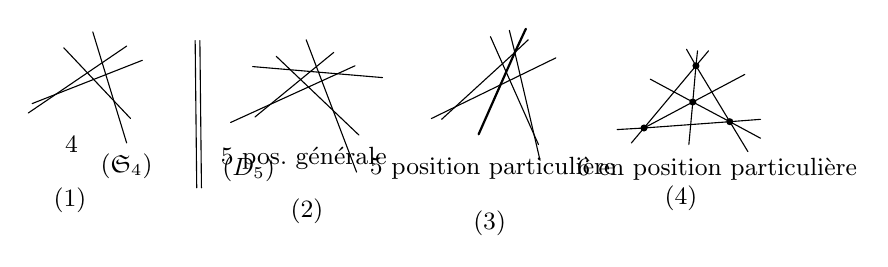
\begin{tikzpicture}[x=1mm,y=1mm,line cap=round,line join=round,font=\scriptsize]
\draw (1.5,-11.5) -- (14,-3);
\draw (2,-10.3) -- (16,-4.8);
\draw (6,-3.2) -- (14.5,-12.2);
\draw (9.7,-1.2) -- (14,-15.3);
\draw (22.7,-2.3) -- (22.9,-21);
\draw (23.3,-2.3) -- (23.5,-21);
\draw (30,-5.6) -- (46.5,-7);
\draw (27.2,-12.7) -- (43,-5.5);
\draw (30.3,-12) -- (40.3,-3.8);
\draw (33,-4.3) -- (43.5,-14.3);
\draw (36.8,-2.2) -- (43.2,-19);
\draw (52.7,-12.2) -- (68.5,-4.5);
\draw (54,-12.3) -- (63.3,-3.8) -- (65,-2.2);
\draw[thick] (58.7,-14.2) -- (63.3,-3.8) -- (64.7,-0.8);
\draw (60.2,-1.8) -- (66.3,-15.5);
\draw (62.6,-1) -- (63.3,-3.8) -- (66.5,-17.5);
\draw (78.1,-15.3) -- (79.7,-13.4) -- (86.3,-5.5) -- (87.9,-3.6);
\draw (85.1,-3.4) -- (86.3,-5.5) -- (90.6,-12.6) -- (92.9,-16.4);
\draw (76.3,-13.6) -- (79.7,-13.4) -- (90.6,-12.6) -- (94.5,-12.3);
\draw (86.5,-3.6) -- (86.3,-5.5) -- (85.9,-10.1) -- (85.4,-15.5);
\draw (79.7,-13.4) -- (85.9,-10.1) -- (92.5,-6.6);
\draw (80.5,-7.2) -- (85.9,-10.1) -- (90.6,-12.6) -- (94.5,-14.7);
\node[pt] at (86.3,-5.5) {};
\node[pt] at (79.7,-13.4) {};
\node[pt] at (90.6,-12.6) {};
\node[pt] at (85.9,-10.1) {};
\node[inner sep=1pt] at (7,-15.5) {\small $4$};
\node[inner sep=1pt] at (14,-18.3) {\small $(\mathfrak{S}_4)$};
\node[inner sep=1pt] at (6.8,-22.6) {\small $(1)$};
\node[inner sep=1pt] at (29.5,-18.7) {\small $(D_5)$};
\node[inner sep=1pt] at (36.5,-17.3) {\small $5$ pos.\ g\'en\'erale};
\node[inner sep=1pt] at (36.9,-24) {\small $(2)$};
\node[inner sep=1pt] at (60.5,-18.5) {\small $5$ position particuli\`ere};
\node[inner sep=1pt] at (60.1,-25.5) {\small $(3)$};
\node[inner sep=1pt] at (89,-18.7) {\small $6$ en position particuli\`ere};
\node[inner sep=1pt] at (84.4,-22.3) {\small $(4)$};
\end{tikzpicture}
\end{document}
